\documentclass[11pt,a4paper]{article}
\usepackage[margin=2.4cm]{geometry}
\usepackage[T1]{fontenc}
\usepackage{lmodern}
\usepackage{graphicx}
\usepackage{booktabs}
\usepackage{tabularx}
\usepackage{caption}
\usepackage{xcolor}
\usepackage[hidelinks]{hyperref}
\usepackage{enumitem}
\usepackage{float}
\usepackage{fancyhdr}
\pagestyle{fancy}\fancyhf{}\cfoot{Page \thepage}\renewcommand{\headrulewidth}{0pt}
\definecolor{navy}{HTML}{0B2A4A}
\setlength{\parskip}{4pt}
\begin{document}
\begin{titlepage}\centering\vspace*{2cm}
{\color{navy}\large Applied AI Research Workshop - Module 2 Methodology and Implementation Report\par}\vspace{0.8cm}
{\color{navy}\LARGE\bfseries Numerical-Text Surrogate Modelling and Multi-Objective Optimisation of Compact Patch Antennas\par}\vspace{0.5cm}
{\large Module 2 of the Applied Vision Transformer Framework for Hybrid-Slotted DGS Antennas in 5G and Emerging 6G Networks - Proof-of-Concept Prototype\par}\vspace{1cm}
{\bfseries Module 2: Numerical-Text Surrogate, Multimodal Fusion and NSGA-II Multi-Objective Optimisation\par}\vspace{2cm}
\begin{tabular}{ll}
\textbf{Student name} & [to be completed by student] \\
\textbf{Student ID} & [to be completed by student] \\
\textbf{Programme / Module} & [to be completed by student] \\
\textbf{Institution} & [to be completed by student] \\
\textbf{Submission date} & [to be completed by student] \\
\textbf{Report generated} & 26 October 2026 \\
\textbf{Code repository} & https://github.com/<your-github-username>/module2-numerical-surrogate-antenna-design \\
\end{tabular}\vfill
{\small Bracketed fields are deliberate placeholders for personal details that were not provided. All results are from executed experiments on public simulation data. Ansys HFSS was not available and was not run.\par}
\end{titlepage}
\tableofcontents\newpage
\section*{Abstract}\addcontentsline{toc}{section}{Abstract}
This report documents the implementation and evaluation of Module 2 of a two-module applied-AI framework for hybrid-slotted defected ground structure (DGS) compact patch antennas. Module 2 is the numerical-text branch: it predicts electromagnetic performance from antenna parameters, turns the predictions into short engineering summaries, fuses numerical features with the image embeddings produced by Module 1, and uses the surrogates inside an NSGA-II multi-objective search. Ansys HFSS was not available, so the module was built and executed on two verified public simulation datasets: 2,051 openEMS rectangular patch antennas (MIT licence) and the Mendeley dual-slot patch Antenna Parameters Dataset (103 designs $\times$ 16 frequencies, CC BY 4.0). On the locked test split shared with Module 1, a random forest predicted the first matched resonance with R$^2$ = 0.89 (MAE 0.35 GHz) and the -10 dB bandwidth with R$^2$ = 0.83, but the depth of the S11 minimum only with R$^2$ = 0.54; all surrogates degraded sharply on wider, out-of-distribution patches. On the slotted Mendeley antenna, grouped cross-validation gave R$^2$ = 0.86 for S11, 0.99 for gain and 0.97 for radiation efficiency, and the geometry variables roughly halved the error of a frequency-only model. The pre-registered fusion hypothesis was not supported: concatenating ViT embeddings with numerical features gave a test macro-F1 of 0.737, against 0.775 for the embeddings alone and 0.716 for the numerical features alone. NSGA-II returned 100 surrogate proposals for the 5G NR n78 band (3.3--3.8 GHz) with areas of 299--2754 mm$^2$. None has been simulated; every proposal and every summary is labelled as requiring full-wave verification.

\textbf{Keywords:} surrogate modelling; random forest; patch antenna; defected ground structure; multimodal fusion; NSGA-II; 5G NR n78.

\section*{1. Introduction and Recap of the Research Problem}\addcontentsline{toc}{section}{1. Introduction and Recap of the Research Problem}
Compact printed patch antennas for 5G and emerging 6G devices are designed by iterating full-wave simulations. Slots and defected ground structures add design freedom but also make the response sensitive to small geometric changes [4], so a parameter sweep in Ansys HFSS can take days. The overall research framework addresses this with two modules. Module 1, documented in a separate report and repository (https://github.com/<your-github-username>/module1-vit-antenna-image-classification), is a Vision Transformer [1] that classifies standardised antenna images. Module 2, documented here, works on numbers: it learns a fast surrogate of the simulator from antenna parameters, explains each prediction in a short engineering summary, combines numerical and image features, and searches the design space for promising candidates. The surrogate is a screening tool that reduces the number of full-wave runs, not a replacement for them.

The objective of Module 2 is \textbf{to determine how well documented antenna parameters predict simulated electromagnetic performance, whether these numbers add to image features, and whether surrogate-based multi-objective optimisation can propose credible compact designs for a 5G band} - while keeping every generated number and sentence traceable to a model output or a simulated reference.

\begin{table}[H]\centering\small
\caption*{Table 1. Implementation status of Module 2.}
\begin{tabularx}{\linewidth}{XXX}
\toprule
\textbf{Component} & \textbf{Status} & \textbf{Evidence in repository} \\
\midrule
Dataset verification, cleaning and plausibility rules & Completed and executed & src/preprocessing.py, docs/DATA\_CARD.md \\
S11 target extraction and locked split (shared with Module 1) & Completed and executed & src/preprocessing.py, data/splits/ \\
Surrogate regression (ridge, gradient boosting, random forest) & Completed and executed & src/numerical\_model.py \\
Rule-based engineering summaries (text) & Completed and executed & results/reports/engineering\_summaries.md \\
Multimodal fusion with Module 1 embeddings & Completed and executed & src/fusion\_optimization.py, results/metrics/fusion.json \\
NSGA-II optimisation for NR n78 & Executed on surrogates only; proposals not simulated & results/metrics/nsga2\_pareto\_n78.csv \\
HFSS hybrid-slotted DGS parameter sweep & Proposed (HFSS unavailable) & Section 11 \\
Full-wave re-simulation, fabrication and measurement & Proposed & Section 11 \\
Block diagram (Figure 1) & Illustrative & results/figures/module2\_architecture.png \\
\bottomrule
\end{tabularx}
\end{table}
\begin{figure}[H]\centering
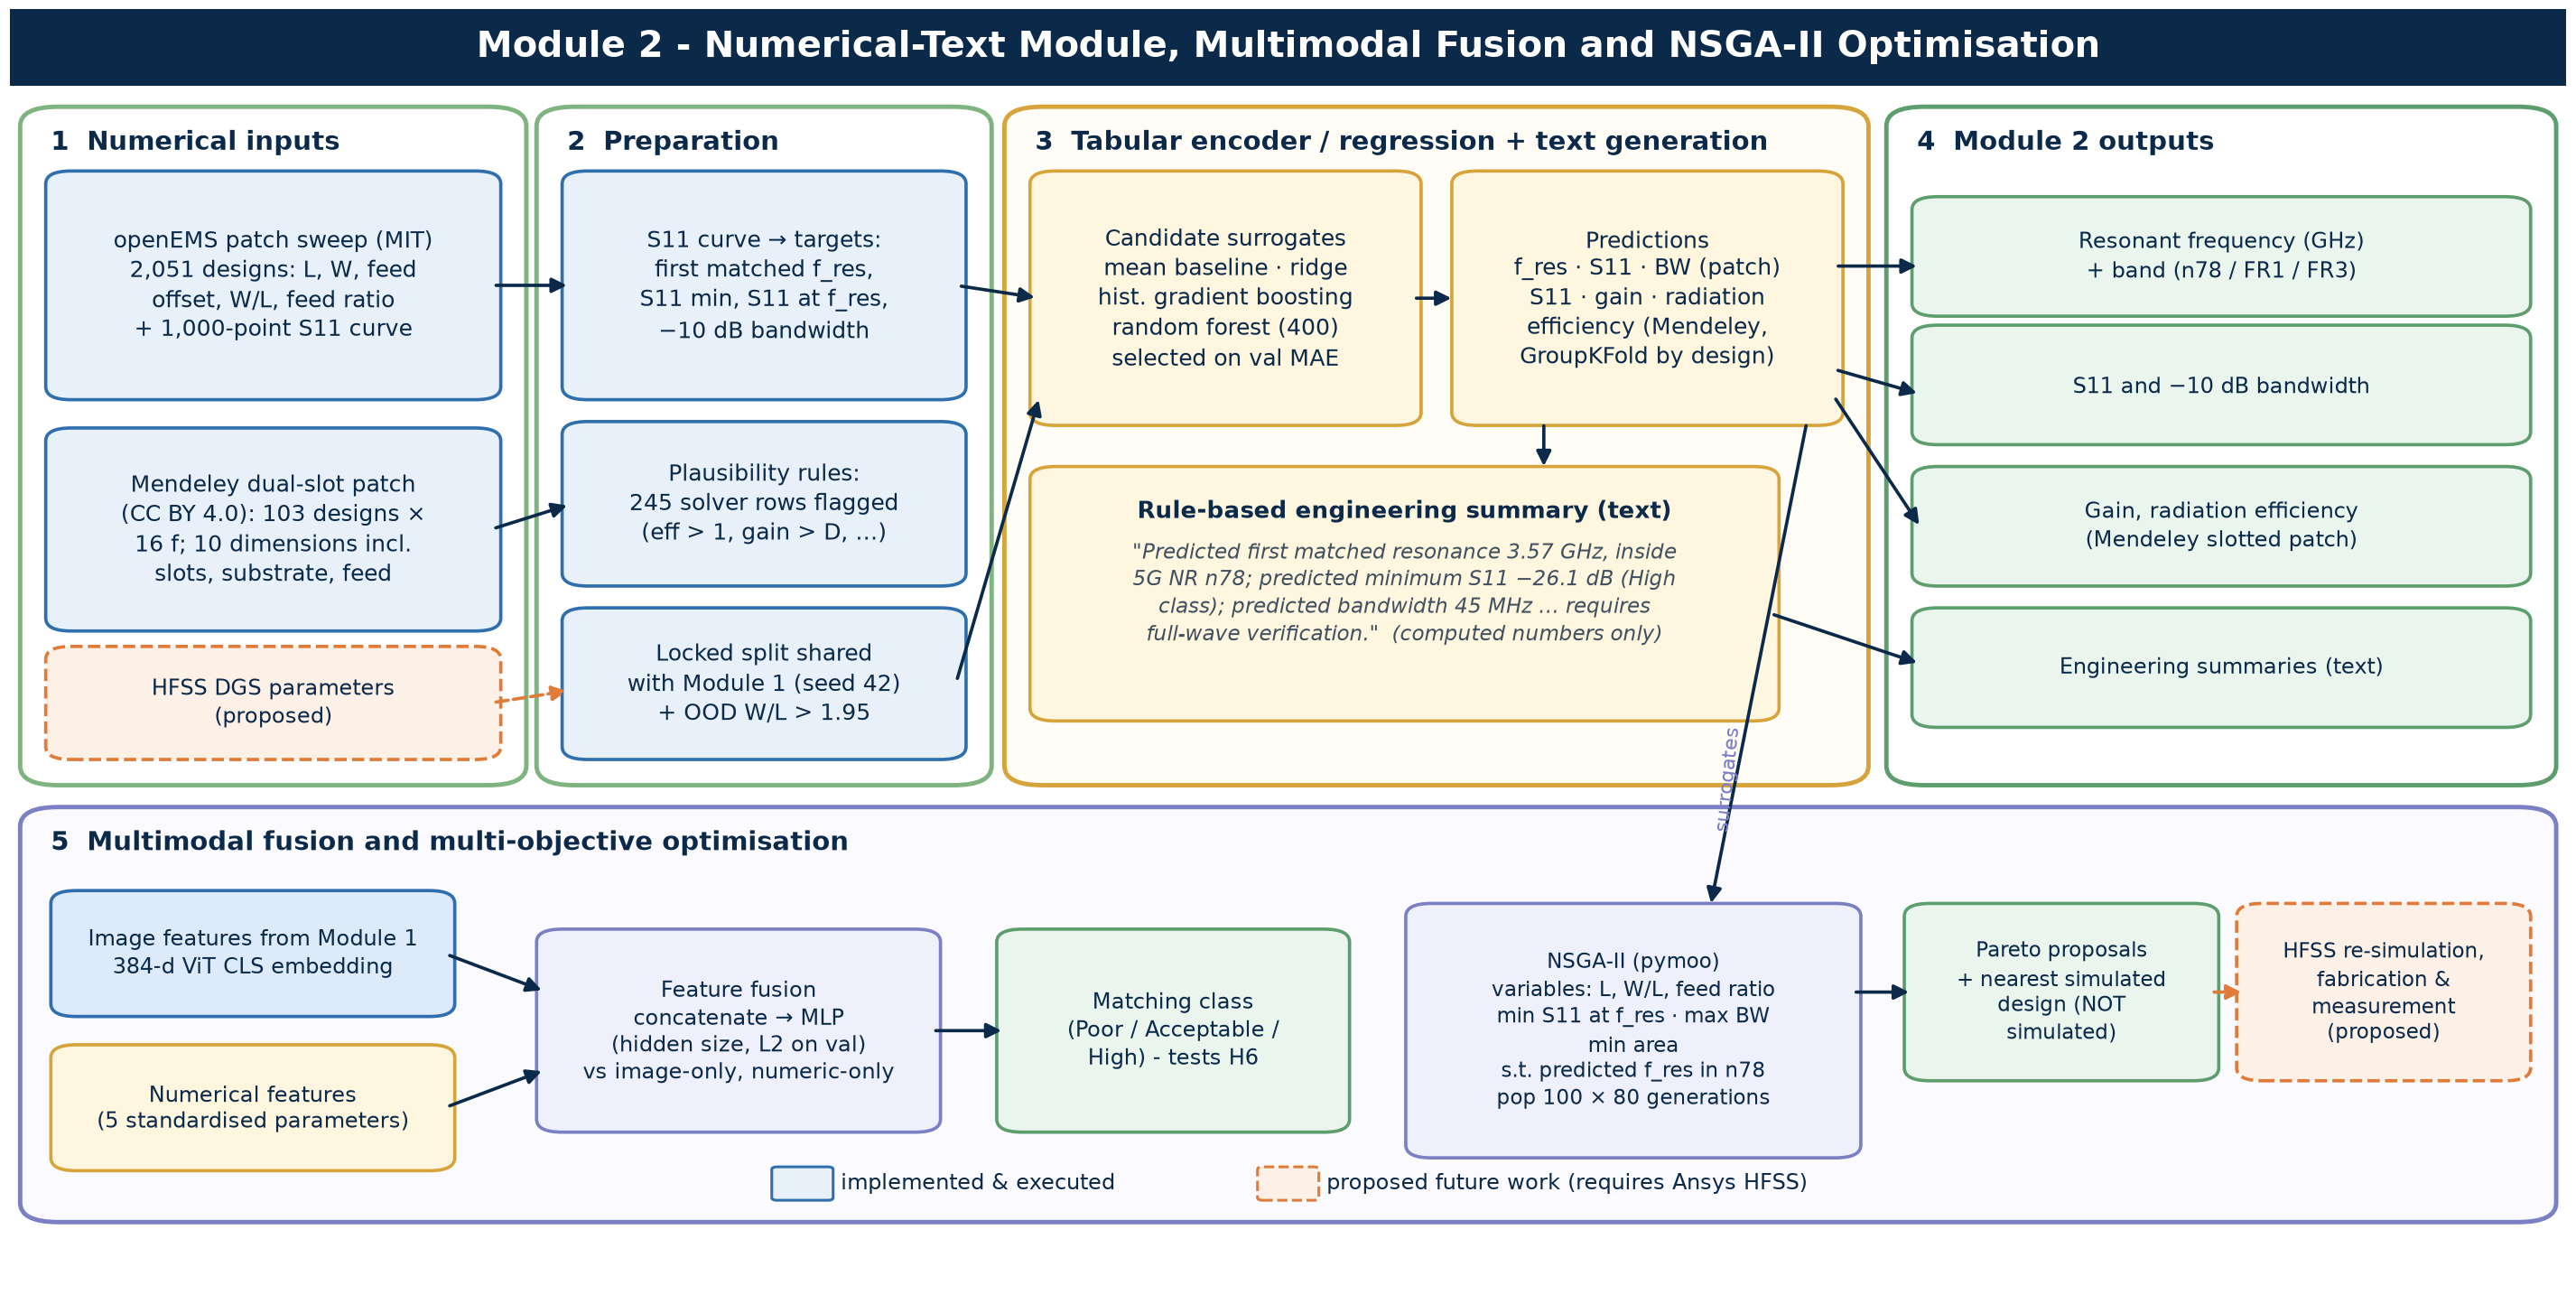
\includegraphics[width=1.00\linewidth]{../results/figures/module2_architecture.png}
\caption*{Figure 1. Module 2 block diagram. Solid boxes were implemented and executed; dashed orange boxes are proposed work that requires Ansys HFSS. The example sentence is a real generated summary.}
\end{figure}
\section*{2. Research Design and Hypotheses}\addcontentsline{toc}{section}{2. Research Design and Hypotheses}
The study follows an applied, experimental machine-learning design. The independent variables are the model family (mean baseline, ridge regression, histogram gradient boosting, random forest, multilayer perceptron), the input set (design geometry, frequency, image embedding, or a combination) and the evaluation distribution (in-distribution test split or out-of-distribution hold-out). The dependent variables are regression errors for continuous targets, classification metrics for the fusion task, and objective values and feasibility for the optimisation.

\begin{table}[H]\centering\small
\caption*{Table 2. Research questions of Module 2 and their operationalisation.}
\begin{tabularx}{\linewidth}{XXX}
\toprule
\textbf{RQ} & \textbf{Question} & \textbf{Operationalisation} \\
\midrule
RQ1 & Can antenna parameters predict simulated resonance, matching and bandwidth? & Patch L, W, feed $\rightarrow$ f\_res, S11min, S11 at f\_res, -10 dB BW; locked test and OOD splits \\
RQ2 & Do slot and substrate dimensions add information beyond frequency? & Mendeley: geometry + frequency vs frequency-only random forest, GroupKFold by design \\
RQ3 & Does fusing image embeddings with numerical features improve classification? & MLP on numeric, image-embedding and concatenated inputs; matching class (H6) \\
RQ4 & Can surrogate-based NSGA-II propose compact, well-matched n78 designs? & Three objectives, band constraint; distance to nearest simulated design \\
RQ5 & Can predictions be summarised in text without inventing values? & Template generator that only verbalises surrogate outputs and dataset references \\
\bottomrule
\end{tabularx}
\end{table}
Hypothesis H6 was pre-registered in Git with the Module 1 hypotheses, before any fusion result existed (docs/HYPOTHESES.md). The other three items below are evaluation criteria stated in the analysis plan; they were not separately pre-registered and are reported as such:

\begin{itemize}[leftmargin=*,itemsep=1pt]
\item \textbf{E1}: Surrogate beats the mean baseline on every patch target (test MAE).
\item \textbf{E2}: Geometry + frequency beats frequency-only (Mendeley, GroupKFold).
\item \textbf{H6}: Fusion (ViT embedding + numeric) > image-only (pre-registered).
\item \textbf{E3}: NSGA-II returns feasible n78 proposals inside the training ranges.
\end{itemize}
\section*{3. Dataset Description and Source Verification}\addcontentsline{toc}{section}{3. Dataset Description and Source Verification}
Repositories were searched in the order set by the brief (Hugging Face, Kaggle, Mendeley Data, IEEE DataPort, GitHub), with Zenodo added; the eleven candidates and the reasons for rejection are recorded in docs/DATASET\_SURVEY.md. Two datasets met the requirements for a numerical module: documented geometric inputs, simulated electromagnetic outputs, a licence that permits reuse, and enough designs for a held-out evaluation. No public HFSS parameter sweep of hybrid-slotted DGS antennas was found.

\begin{table}[H]\centering\small
\caption*{Table 3. Datasets used by Module 2 (verified 25 October 2026).}
\begin{tabularx}{\linewidth}{XXXXX}
\toprule
\textbf{Dataset} & \textbf{Source / version} & \textbf{Licence} & \textbf{Content} & \textbf{Role in Module 2} \\
\midrule
Rectangular Patch Antenna Frequency Response [2] & Hugging Face becklabash/rectangular-patch-antenna-freq-response, rev. 4be72a2 & MIT & 2,051 coax-fed patches; L, W, feed offset; 1,000-point S11 (1--10 GHz), openEMS FDTD [11]; $\varepsilon$r 3.68, h 1.61 mm & Surrogate targets, fusion, NSGA-II \\
Antenna Parameters Dataset [3] & Mendeley Data 10.17632/3gxr2vvd9n.2 & CC BY 4.0 & 103 dual-slot patch designs $\times$ 16 frequencies (1--50 GHz): S11, gain, directivity, efficiencies, VSWR & Slotted-antenna regression (S11, gain, efficiency) \\
Module 1 image embeddings & Module 1 repository, run vit\_finetune\_patch\_perf\_class\_s42 & Derived (MIT data) & 384-d ViT CLS embedding per patch design; SHA-256 recorded & Image features for fusion only \\
\bottomrule
\end{tabularx}
\end{table}
\textbf{Nature of the evidence.} Both datasets are full-wave simulations; neither contains measurements, and no HFSS output is claimed. The Mendeley data are one-at-a-time sweeps around a single nominal design, so most designs differ from the nominal one in a single dimension. The Module 1 embeddings were produced by a ViT fine-tuned on the training split only; validation, test and OOD images were never used to fit it (data/external/module1\_vit\_embeddings/provenance.json).

\textbf{Discrepancies recorded during verification.} The patch README gives L $\in$ [7.5, 52.5] mm and p $\in$ [-6, 0) mm; the observed values are L $\in$ [7.5, 47.5] mm and p $\in$ [-15.83, 0] mm, including 100 centre-fed designs. The README states $\varepsilon$r = 3.68 while the repository diagram shows 3.38. 1170 S11 curves exceed 0 dB by at most 0.2 dB, a passive-port numerical artefact. In the Mendeley data, 245 of 1,648 rows are physically implausible and one efficiency entry is a truncated, non-numeric string. The reference report cites Mendeley version 1, which has since been superseded by version 2.

\section*{4. Data Preprocessing and Preparation}\addcontentsline{toc}{section}{4. Data Preprocessing and Preparation}
\subsection*{4.1 Engineering targets from simulated S11}\addcontentsline{toc}{subsection}{4.1 Engineering targets from simulated S11}
Each 1,000-point S11 curve was reduced to four regression targets: the global minimum S11 (S11min); the \textbf{first matched resonance} f\_res, defined as the lowest-frequency local minimum below -10 dB; S11 at f\_res; and the contiguous -10 dB bandwidth around f\_res. The first matched resonance is used because the deepest dip is often a higher-order mode; a 22.5 mm patch, for example, has its deepest dip at 9.6 GHz. Unmatched designs keep the global minimum as f\_res and a bandwidth of 0. The same rules define the matching class used in the fusion task (Poor if S11min > -10 dB, Acceptable if -20 dB < S11min $\leq$ -10 dB, High if S11min $\leq$ -20 dB). The -20 dB boundary is a \textbf{project assumption} that requires engineering confirmation.

\begin{figure}[H]\centering
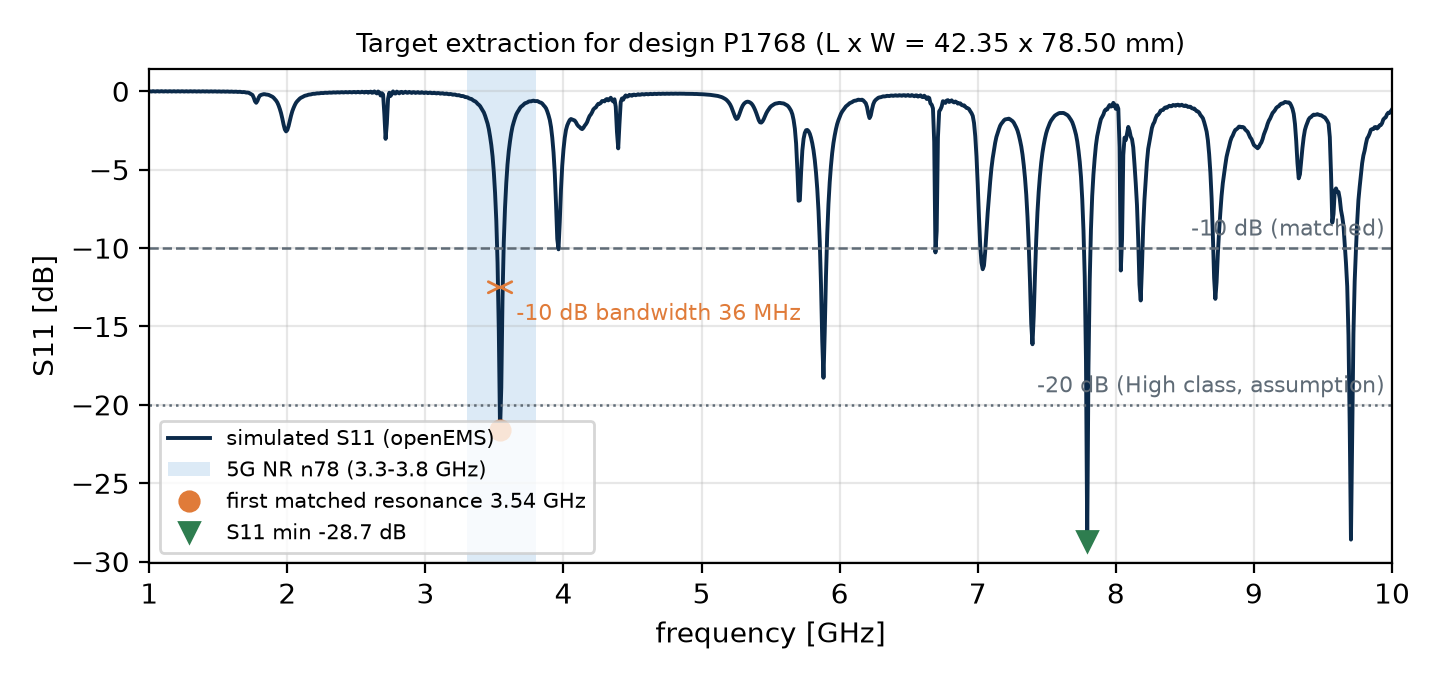
\includegraphics[width=0.95\linewidth]{../results/figures/s11_target_extraction.png}
\caption*{Figure 2. How the regression targets are extracted from one simulated S11 curve (test design P1768). The deepest dip lies outside n78; the first matched resonance lies inside it.}
\end{figure}
\subsection*{4.2 Cleaning and plausibility rules}\addcontentsline{toc}{subsection}{4.2 Cleaning and plausibility rules}
\begin{itemize}[leftmargin=*,itemsep=1pt]
\item Patch: 2,051 rows, 0 non-finite curves, 0 duplicate parameter triples and 0 missing values after feature extraction. Extreme S11 values are physical deep matches and were kept.
\item Mendeley: column names were stripped and normalised, the non-numeric efficiency entry was set to missing, and every row was assigned a design ID from its ten geometry variables (103 designs $\times$ 16 frequencies; 0 duplicate rows).
\item Plausibility rule (documented, not tuned): a row is flagged if radiation or total efficiency exceeds 1, directivity exceeds 20 dBi for an antenna of about 6 mm, or gain exceeds directivity. 245 rows were flagged; they are excluded from the gain and efficiency targets (1,403 rows remain) but kept for S11, which they do not affect.
\end{itemize}
\subsection*{4.3 Features, split and leakage control}\addcontentsline{toc}{subsection}{4.3 Features, split and leakage control}
\begin{itemize}[leftmargin=*,itemsep=1pt]
\item Patch inputs: length L, width W, feed offset, aspect ratio W/L and normalised feed position (feed offset / (L/2)). Mendeley inputs: the ten substrate, patch, feed and slot dimensions plus frequency.
\item Split: Module 2 reproduces the locked design-level split of Module 1 and verifies it against the committed manifests (train 1,220, validation 262, test 262, OOD hold-out 307 with W/L > 1.95). This keeps the fusion comparison fair and makes the two modules' test results refer to the same designs.
\item Mendeley evaluation uses 5-fold GroupKFold by design, so all 16 frequencies of one design are always in the same fold.
\item Standardisation statistics (ridge, MLP) are fitted on training data only; tree models need no scaling.
\item The test split is scored once, after model selection on validation MAE (regression) or validation macro-F1 (fusion).
\end{itemize}
The data dictionary is in Appendix A; all counts are logged in data/processed/preprocessing\_log.json and results/metrics/mendeley\_cleaning.json, and the rules are enforced by automated tests (Section 10).

\section*{5. Proposed Model: Numerical-Text Surrogate, Fusion and Optimisation}\addcontentsline{toc}{section}{5. Proposed Model: Numerical-Text Surrogate, Fusion and Optimisation}
\textbf{Tabular surrogate.} For each target, four candidates are trained: a mean predictor, ridge regression [12], histogram gradient boosting [7] and a random forest of 400 trees [6], all from scikit-learn [8]. The candidate with the lowest validation MAE is selected. Tree ensembles suit this problem: the response is non-linear and non-additive (the resonance depends on length, the match on the feed position relative to the edge), and the datasets are small. Permutation importance on the validation split [13] shows which inputs each surrogate relies on.

\textbf{Text generation.} The engineering summary is produced by a deterministic template, not by a language model. It reads the surrogate's predictions and the dataset's simulated reference for the same design, maps them to the band (n78, FR1 or FR3 [5]) and to the matching rule, and writes one paragraph. Because every number in the sentence is copied from a computed value, the generator cannot invent a measurement, and each summary ends with the statement that full-wave verification is required.

\textbf{Multimodal fusion.} The 384-dimensional CLS embedding exported by Module 1 and the five standardised numerical features are concatenated and classified by a multilayer perceptron [14] into the three matching classes. Two reference models use the embedding only and the numerical features only. Hidden size ((64) or (128, 64)) and L2 penalty (1e-4, 1e-3, 1e-2) are chosen on validation macro-F1 for each variant. This is the early-fusion design of the framework figure [15].

\textbf{Multi-objective optimisation.} NSGA-II [9], implemented in pymoo [10], searches three decision variables - patch length L, aspect ratio W/L and normalised feed position - bounded by their observed training ranges. It minimises predicted S11 at resonance, maximises predicted -10 dB bandwidth and minimises patch area, subject to the predicted first matched resonance lying in 5G NR band n78 (3.3--3.8 GHz). Population size is 100 and the search runs for 80 generations. Each Pareto proposal is reported with its nearest simulated design in standardised parameter space, as a check on how far the surrogate is extrapolating.

\section*{6. Training Strategy and Experimental Setup}\addcontentsline{toc}{section}{6. Training Strategy and Experimental Setup}
\begin{table}[H]\centering\small
\caption*{Table 4. Module 2 configuration (configs/default.yaml).}
\begin{tabularx}{\linewidth}{XXX}
\toprule
\textbf{Component} & \textbf{Setting} & \textbf{Selection / note} \\
\midrule
Random forest & 400 trees, unlimited depth, min. 1 sample per leaf & Seed 42; candidate per target \\
Histogram gradient boosting & 500 iterations, learning rate 0.05 & Seed 42; candidate per target \\
Ridge regression & α = 1.0, standardised inputs & Linear reference \\
Model selection (patch) & Lowest validation MAE per target & Test scored once \\
Mendeley evaluation & 5-fold GroupKFold by design & Out-of-fold predictions \\
Fusion MLP & Adam, $\leq$ 800 iterations; hidden (64) or (128, 64); α $\in$ \{1e-4, 1e-3, 1e-2\} & Chosen on validation macro-F1 \\
NSGA-II & Population 100, 80 generations, 3 objectives, 2 constraints & Seed 42 \\
Hardware & Intel i7-10610U CPU & Full Module 2 pipeline runs in a few minutes \\
\bottomrule
\end{tabularx}
\end{table}
No hyperparameter of the tree models was tuned beyond the candidate comparison, because the aim is a robust baseline surrogate rather than a leaderboard result; the configuration is fixed in one file and every run is seeded.

\section*{7. Baseline Methods and Comparative Models}\addcontentsline{toc}{section}{7. Baseline Methods and Comparative Models}
\begin{itemize}[leftmargin=*,itemsep=1pt]
\item \textbf{Mean baseline}: predicts the training mean of each target; any useful surrogate must beat it.
\item \textbf{Ridge regression}: a linear model on standardised inputs; shows how much of the response is linear.
\item \textbf{Frequency-only random forest} (Mendeley): the same model given only frequency, isolating the contribution of the geometry.
\item \textbf{Image-only and numeric-only MLPs} (fusion): the two single-modality references for H6.
\item \textbf{Module 1 ViT linear head}: the fine-tuned ViT's own classifier, test macro-F1 0.581 (reported by Module 1), for context on the image-only MLP.
\item \textbf{Simulated designs in band} (optimisation): the best simulated n78 designs in the dataset, as a reference for the Pareto set.
\end{itemize}
\section*{8. Evaluation Metrics and Analysis Plan}\addcontentsline{toc}{section}{8. Evaluation Metrics and Analysis Plan}
Regression is reported with mean absolute error (MAE), root mean squared error (RMSE) and the coefficient of determination R$^2$, on the locked test split and separately on the OOD hold-out. For the Mendeley data the metrics are computed on pooled out-of-fold predictions. The fusion task uses macro-F1 (primary, because the classes are imbalanced), accuracy, balanced accuracy, one-vs-rest macro ROC-AUC and the confusion matrix. The optimisation is described by the number of non-dominated proposals, the ranges of the objectives, constraint satisfaction and the distance of each proposal to its nearest simulated design. The analysis plan and H6 were fixed before results were produced.

\section*{9. Results and Discussion}\addcontentsline{toc}{section}{9. Results and Discussion}
Every number in this section comes from executed runs stored in results/metrics. No value is estimated or illustrative.

\subsection*{9.1 Patch surrogate: resonance, matching and bandwidth (RQ1)}\addcontentsline{toc}{subsection}{9.1 Patch surrogate: resonance, matching and bandwidth (RQ1)}
\begin{table}[H]\centering\small
\caption*{Table 5. Patch surrogate, locked test split (n = 262 designs) and OOD hold-out (n = 307); model selected on validation MAE.}
\begin{tabularx}{\linewidth}{XXXXXXX}
\toprule
\textbf{Target} & \textbf{Model} & \textbf{Test MAE} & \textbf{Test RMSE} & \textbf{Test R$^2$} & \textbf{Mean-baseline MAE} & \textbf{OOD R$^2$} \\
\midrule
First matched resonance (GHz) & random forest & 0.355 & 0.739 & 0.888 & 1.820 & 0.444 \\
Minimum S11 (dB) & random forest & 4.815 & 6.421 & 0.538 & 7.363 & 0.132 \\
S11 at resonance (dB) & random forest & 3.272 & 4.998 & 0.570 & 5.648 & -1.544 \\
-10 dB bandwidth (MHz) & random forest & 18.056 & 34.371 & 0.830 & 55.361 & -3.723 \\
\bottomrule
\end{tabularx}
\end{table}
\begin{figure}[H]\centering
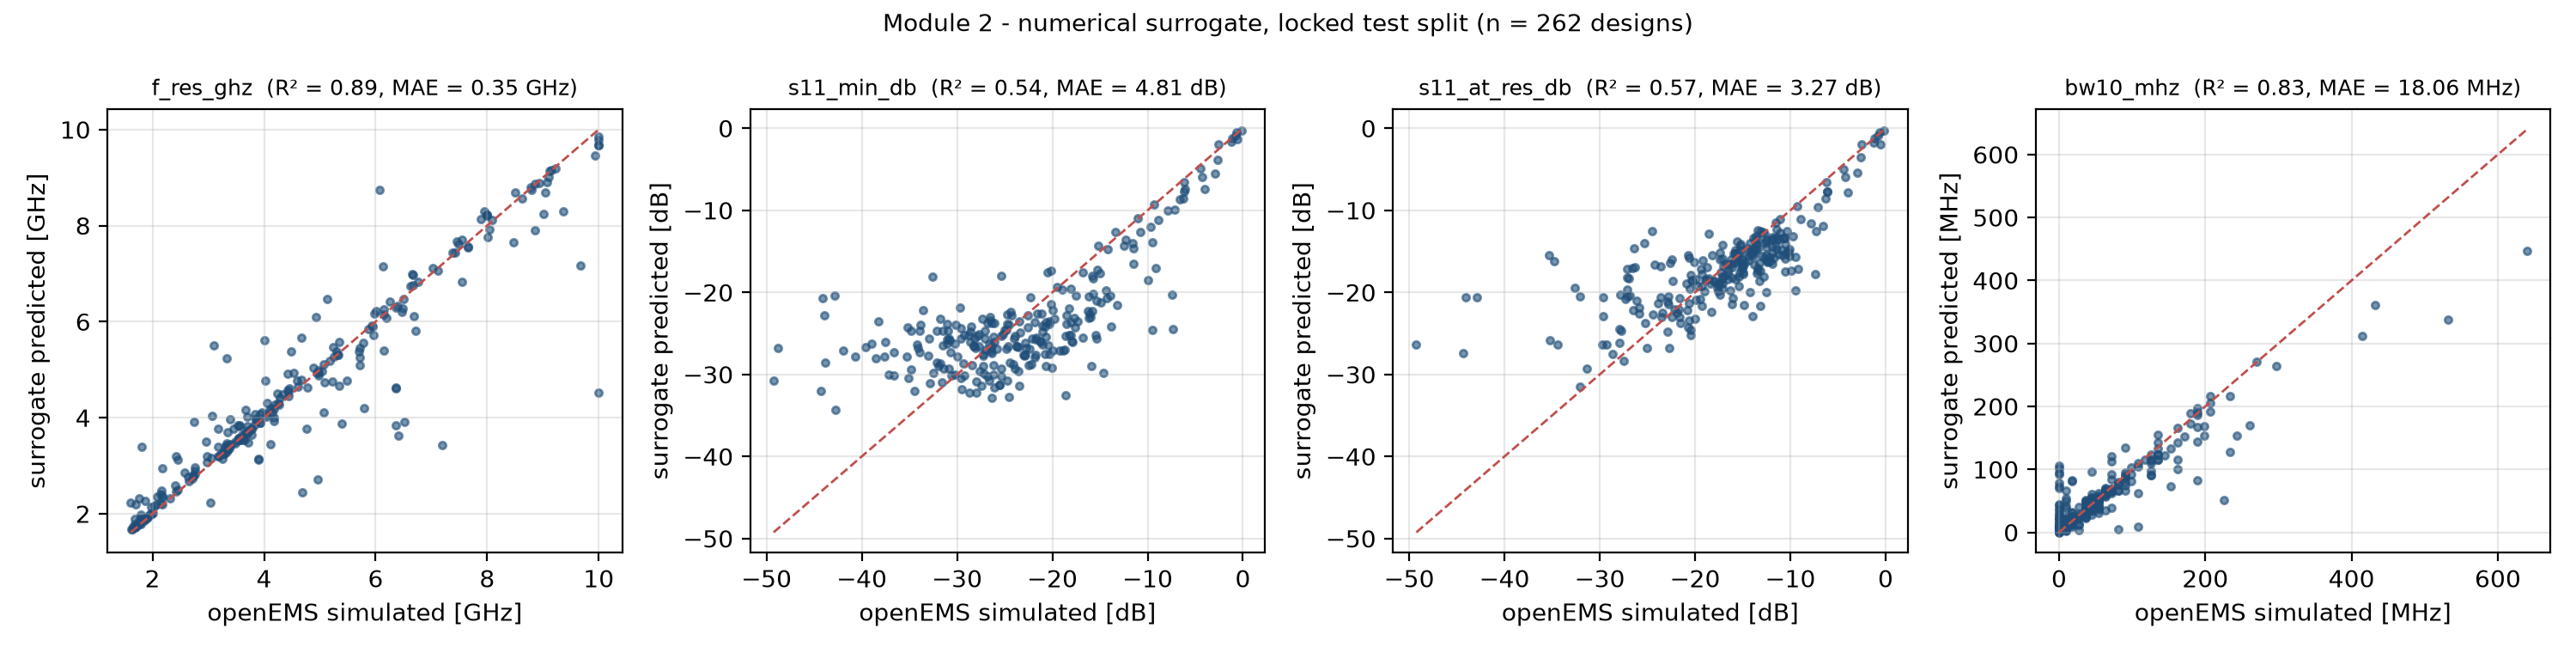
\includegraphics[width=1.00\linewidth]{../results/figures/numerical_parity_patch.png}
\caption*{Figure 3. Parity plots of the selected surrogates on the locked patch test split.}
\end{figure}
\begin{figure}[H]\centering
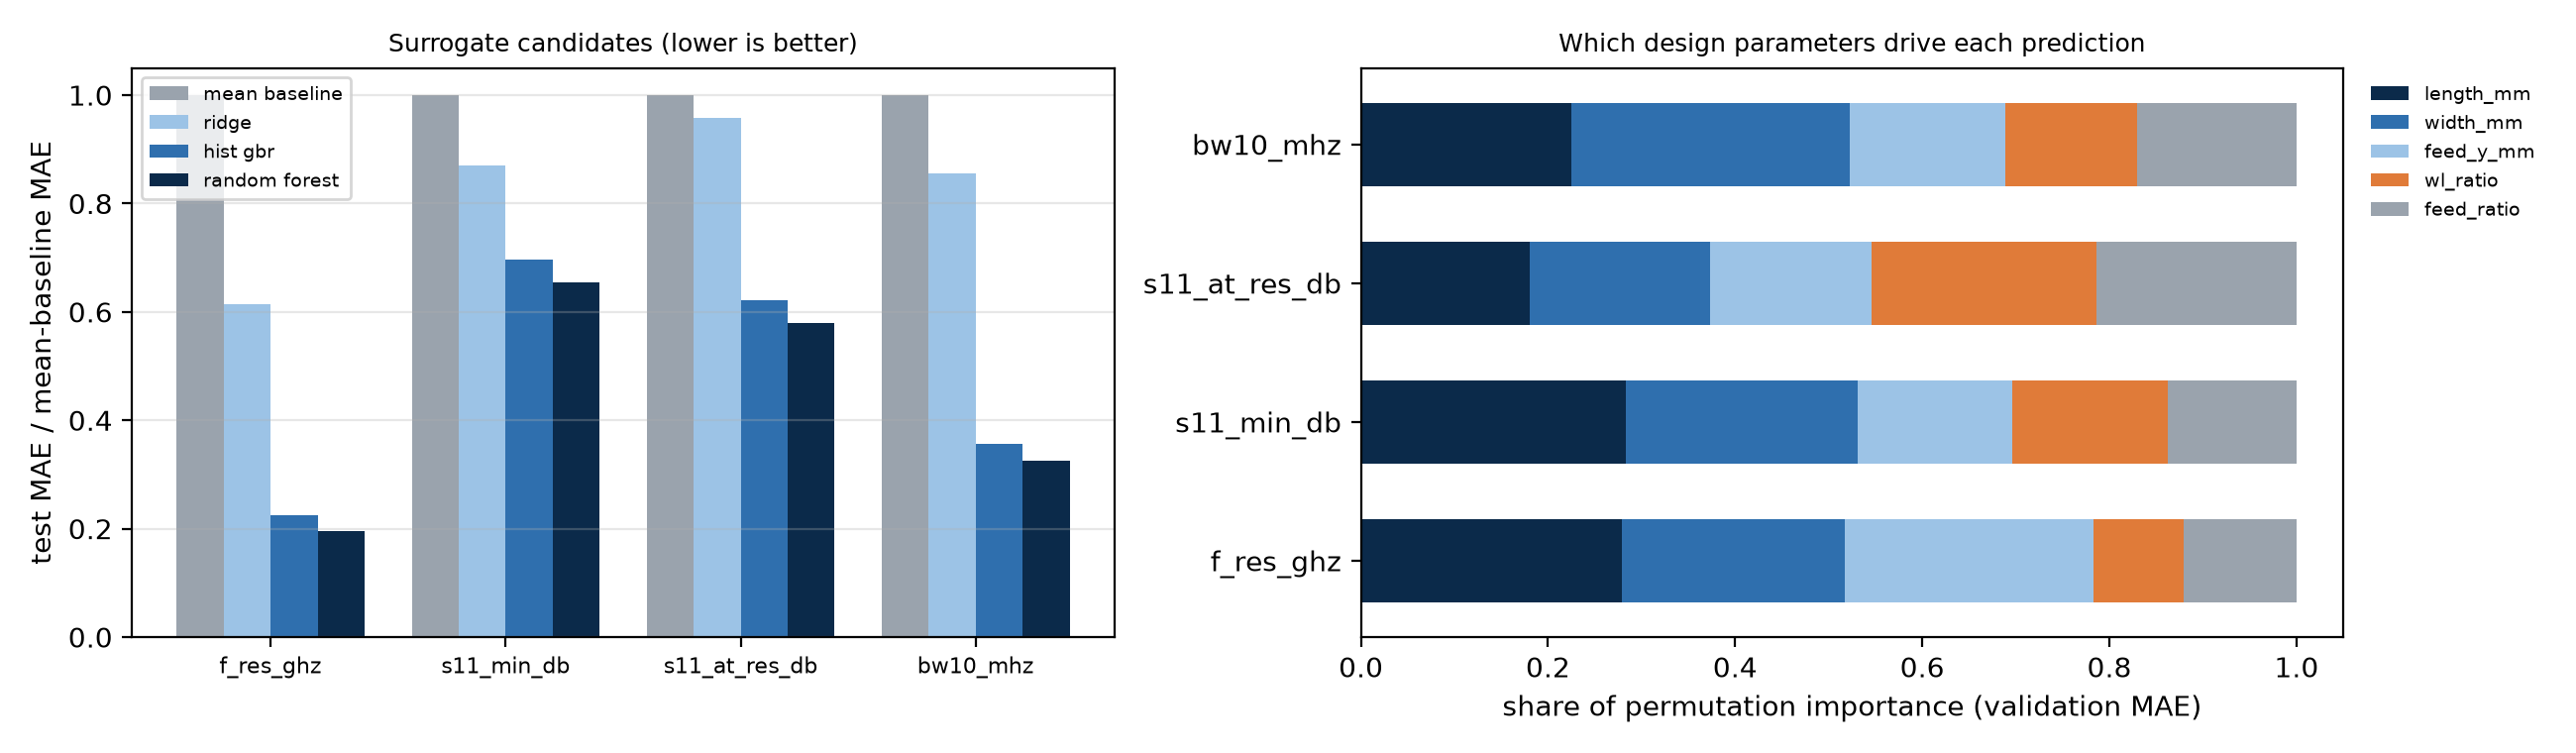
\includegraphics[width=1.00\linewidth]{../results/figures/surrogate_comparison_importance.png}
\caption*{Figure 4. Left: test MAE of each candidate relative to the mean baseline. Right: share of permutation importance (validation MAE) per input.}
\end{figure}
The random forest was selected for all four targets and beat the mean baseline on each (\textbf{E1} -- Met: all four targets; weakest s11\_min\_db (4.81 vs 7.36)). It predicts the first matched resonance well (R$^2$ = 0.89, MAE 0.35 GHz) and the -10 dB bandwidth well (R$^2$ = 0.83, MAE 18.1 MHz). It predicts the depth of the S11 minimum only moderately (R$^2$ = 0.54, MAE 4.8 dB). This is physically reasonable: resonance varies smoothly with patch length [4], whereas the depth of the match is a sharp function of how closely the input impedance at the feed approaches the 50 Ω port, so small parameter changes produce large changes in dB. The same sharpness explains why the matching class is the hardest task for the image models of Module 1. Ridge regression captured little of any target, confirming that the response is strongly non-linear. Permutation importance spread across all five inputs; length was the most important input for 2 of the four targets, as expected from the half-wavelength resonance condition.

\textbf{Out-of-distribution behaviour.} On the wider patches of the OOD hold-out, R$^2$ fell to 0.44 for the resonance and below zero for S11 at resonance (-1.54) and bandwidth (-3.72). Tree ensembles cannot extrapolate beyond the training range, and wide patches excite different modes. This is the most important caveat for the optimisation stage: surrogate predictions are only trustworthy close to simulated designs, which is why the NSGA-II search is bounded by the training ranges and each proposal is checked against its nearest simulated neighbour.

\subsection*{9.2 Slotted patch: S11, gain and efficiency (RQ2)}\addcontentsline{toc}{subsection}{9.2 Slotted patch: S11, gain and efficiency (RQ2)}
\begin{table}[H]\centering\small
\caption*{Table 6. Mendeley dual-slot patch, 5-fold GroupKFold by design (out-of-fold predictions).}
\begin{tabularx}{\linewidth}{XXXXX}
\toprule
\textbf{Target} & \textbf{Model} & \textbf{MAE} & \textbf{RMSE} & \textbf{R$^2$} \\
\midrule
S11 (dB) & mean baseline & 3.790 & 6.092 & -0.000 \\
S11 (dB) & ridge & 3.254 & 5.822 & 0.086 \\
S11 (dB) & hist gbr & 0.701 & 2.039 & 0.888 \\
S11 (dB) & random forest & 0.533 & 2.299 & 0.858 \\
S11 (dB) & random forest frequency only & 1.089 & 3.059 & 0.748 \\
Gain (dBi) & mean baseline & 9.652 & 13.126 & -0.000 \\
Gain (dBi) & ridge & 6.556 & 8.656 & 0.565 \\
Gain (dBi) & hist gbr & 0.797 & 1.475 & 0.987 \\
Gain (dBi) & random forest & 0.513 & 1.241 & 0.991 \\
Gain (dBi) & random forest frequency only & 1.096 & 1.904 & 0.979 \\
Radiation efficiency (ratio) & mean baseline & 0.299 & 0.344 & -0.000 \\
Radiation efficiency (ratio) & ridge & 0.132 & 0.157 & 0.790 \\
Radiation efficiency (ratio) & hist gbr & 0.037 & 0.068 & 0.961 \\
Radiation efficiency (ratio) & random forest & 0.026 & 0.061 & 0.969 \\
Radiation efficiency (ratio) & random forest frequency only & 0.047 & 0.083 & 0.942 \\
\bottomrule
\end{tabularx}
\end{table}
\begin{figure}[H]\centering
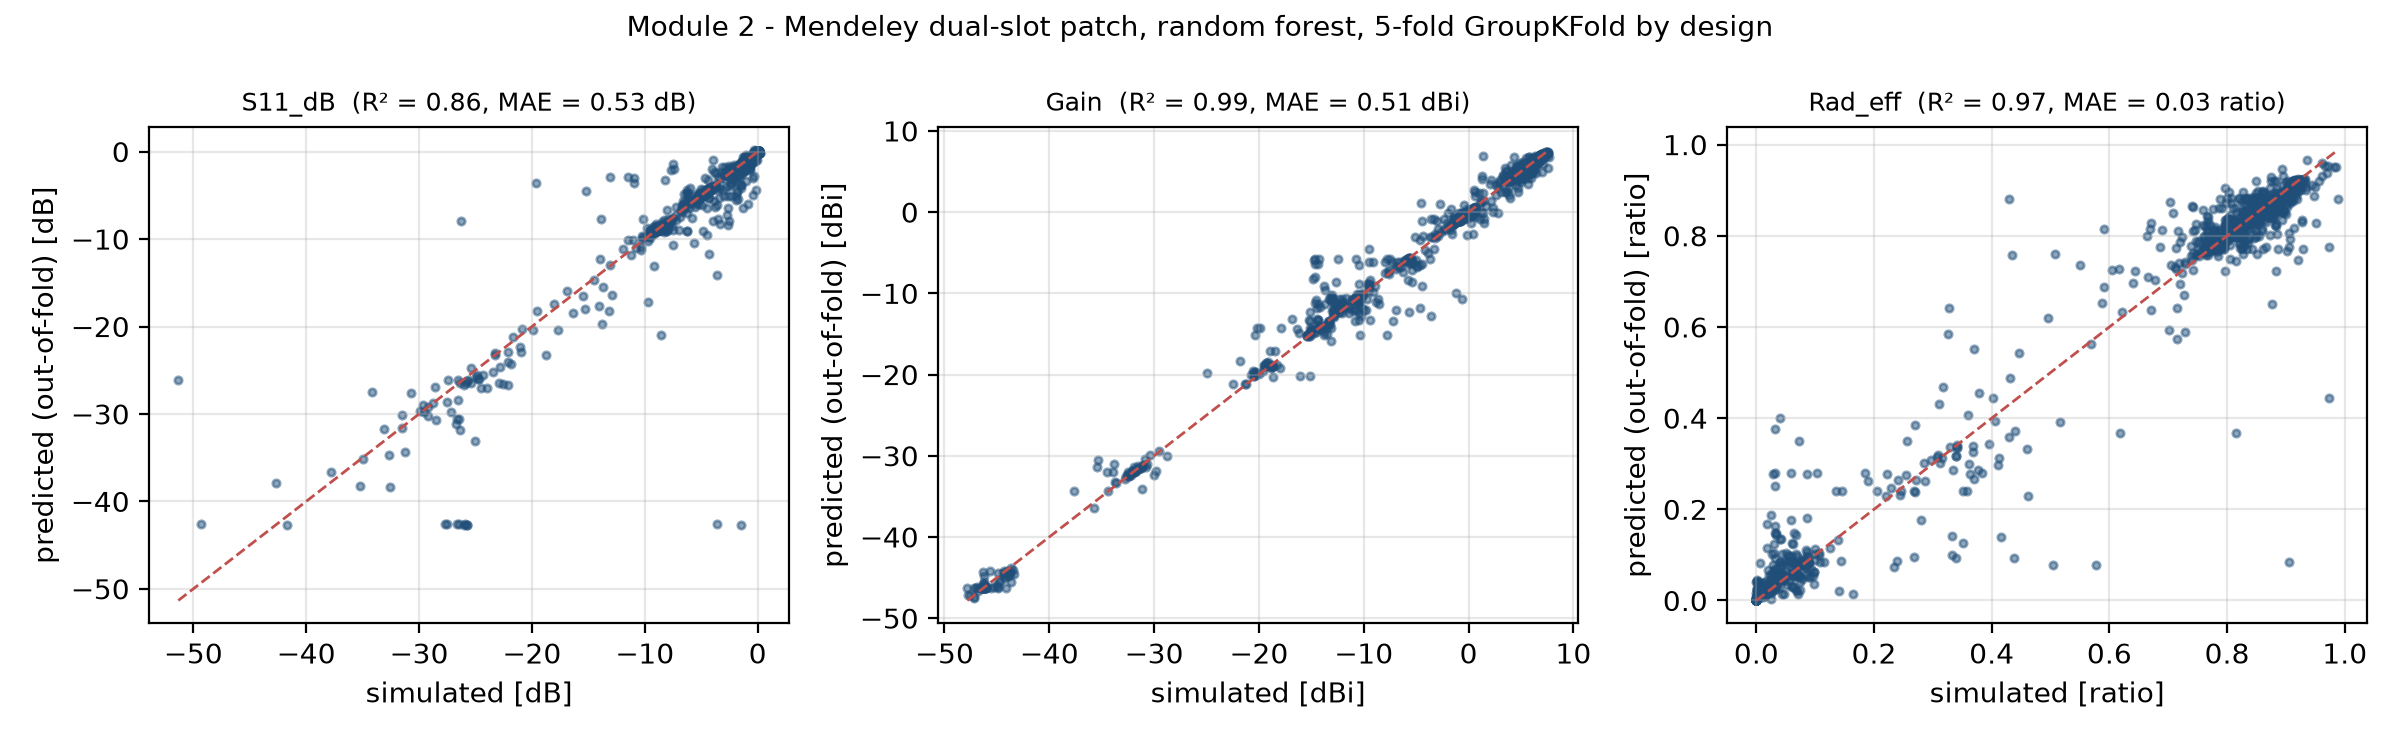
\includegraphics[width=1.00\linewidth]{../results/figures/numerical_parity_mendeley.png}
\caption*{Figure 5. Out-of-fold parity plots for the random forest on the Mendeley dual-slot patch.}
\end{figure}
Adding the ten geometry variables to frequency reduced the random-forest error for every target (\textbf{E2} -- Met: S11\_dB 0.533 vs 1.089; Gain 0.513 vs 1.096; Rad\_eff 0.026 vs 0.047). The very high gain and efficiency R$^2$ mostly reflect the strong frequency dependence over 1--50 GHz: the frequency-only model already reaches R$^2$ = 0.98 for gain. Because the data are one-at-a-time sweeps around one nominal design, the geometry effect is estimated from a narrow neighbourhood and the grouped folds still contain near-identical designs, so these scores overstate how well the model would generalise to a new slot topology. S11 is the hardest target here as well: a few deep resonances are badly under- or over-predicted, which is visible as horizontal clusters in the parity plot.

\subsection*{9.3 Engineering summaries (RQ5)}\addcontentsline{toc}{subsection}{9.3 Engineering summaries (RQ5)}
The text generator wrote one summary per selected test design and per highlighted Pareto proposal (results/reports/engineering\_summaries.md). Two unedited examples:

\begin{itemize}[leftmargin=*,itemsep=1pt]
\item P1768 - patch L x W = 42.35 x 78.50 mm (W/L 1.85), feed offset -1.89 mm. Predicted first matched resonance 3.57 GHz, inside 5G NR n78 (3.3-3.8 GHz, FR1); predicted minimum S11 -26.1 dB, which meets the -20 dB project threshold (High class); predicted -10 dB bandwidth 45 MHz. Simulated reference (openEMS): 3.54 GHz, -28.7 dB, 36 MHz. Status: surrogate screening only - requires full-wave verification.
\item N78-001 (smallest area) - patch L x W = 19.31 x 15.48 mm (area 299 mm$^2$, W/L 0.80), feed offset -2.89 mm. Predicted first matched resonance 3.79 GHz, inside 5G NR n78 (3.3-3.8 GHz, FR1); predicted S11 at resonance -26.6 dB, which meets the -20 dB project threshold (High class); predicted -10 dB bandwidth 64 MHz. Nearest simulated design P0564 (0.07 standard units away) resonates at 3.82 GHz with -28.6 dB and 63 MHz. Status: surrogate proposal - NOT simulated; requires full-wave verification.
\end{itemize}
Each sentence places the predicted values next to the simulated reference, so a reader can see the surrogate error directly (in the first example the resonance is predicted within a few tens of MHz). The generator never produces a number that the model or the dataset did not produce, and it never states that a design is verified. Its limitation is expressiveness: it cannot explain why a design behaves as it does, only restate the numbers in engineering terms.

\subsection*{9.4 Multimodal fusion (RQ3, H6)}\addcontentsline{toc}{subsection}{9.4 Multimodal fusion (RQ3, H6)}
\begin{table}[H]\centering\small
\caption*{Table 7. Fusion experiment, matching class (MLP; configuration selected on validation macro-F1).}
\begin{tabularx}{\linewidth}{XXXXXXX}
\toprule
\textbf{Input} & \textbf{Features} & \textbf{Val macro-F1} & \textbf{Test macro-F1} & \textbf{Test bal. acc.} & \textbf{Test ROC-AUC} & \textbf{OOD macro-F1} \\
\midrule
numeric only & 5 & 0.742 & 0.716 & 0.691 & 0.876 & 0.581 \\
image only & 384 & 0.787 & 0.775 & 0.757 & 0.888 & 0.608 \\
fusion concat & 389 & 0.766 & 0.737 & 0.716 & 0.876 & 0.611 \\
\bottomrule
\end{tabularx}
\end{table}
\begin{figure}[H]\centering
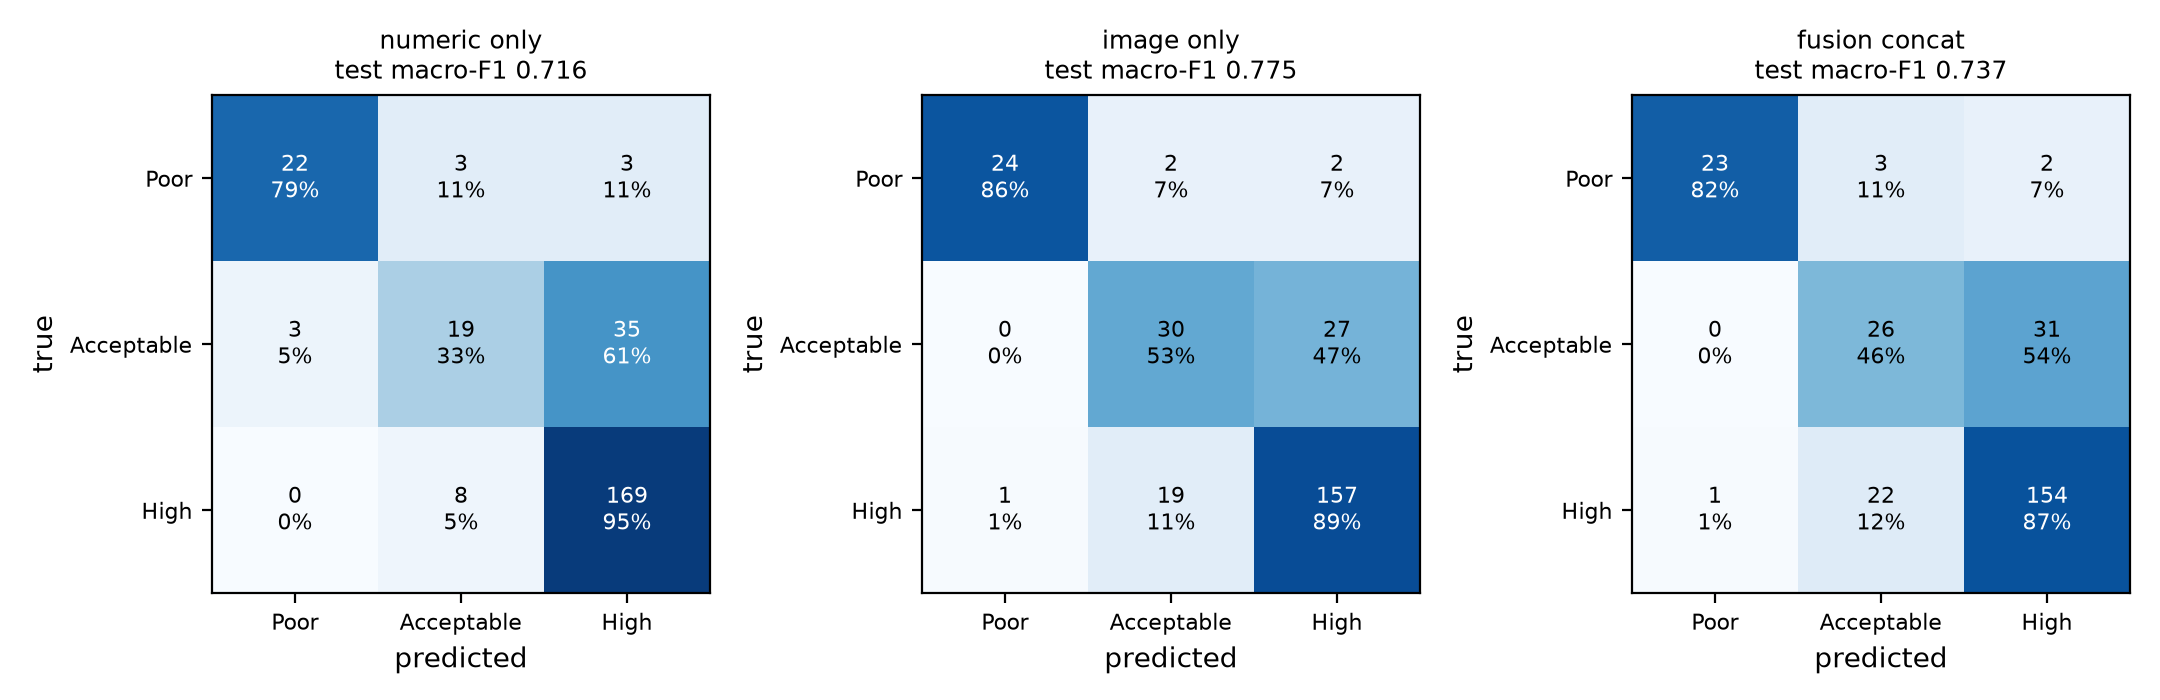
\includegraphics[width=0.95\linewidth]{../results/figures/fusion_confusion.png}
\caption*{Figure 6. Test confusion matrices of the three fusion variants.}
\end{figure}
\textbf{H6} -- Not supported: 0.737 vs 0.775 (numeric-only 0.716). Concatenating the five numerical features with the 384-d image embedding lowered test macro-F1 compared with the embedding alone, so the pre-registered hypothesis is not supported. The most informative result is the image-only MLP: trained on frozen embeddings of the fine-tuned ViT it reached 0.775, far above the ViT's own linear head (0.581, Module 1). This supports Module 1's underfitting diagnosis - the representation captured the relevant geometry, but the end-to-end head did not converge within the CPU budget. The numeric-only MLP (0.716) was weaker than image-only although the five parameters fully determine each design; a small MLP underfits the sharp S11 dependence, whereas the embedding already encodes size and feed position. Adding the numbers to 384 image dimensions mainly added redundant inputs for a small training set. The embeddings were fitted on the same training labels, so training-set features are optimistic; validation and test images were never used for fitting, so the test numbers remain valid, but the comparison should be confirmed with cross-fitted embeddings.

\subsection*{9.5 NSGA-II surrogate optimisation for NR n78 (RQ4)}\addcontentsline{toc}{subsection}{9.5 NSGA-II surrogate optimisation for NR n78 (RQ4)}
\begin{figure}[H]\centering
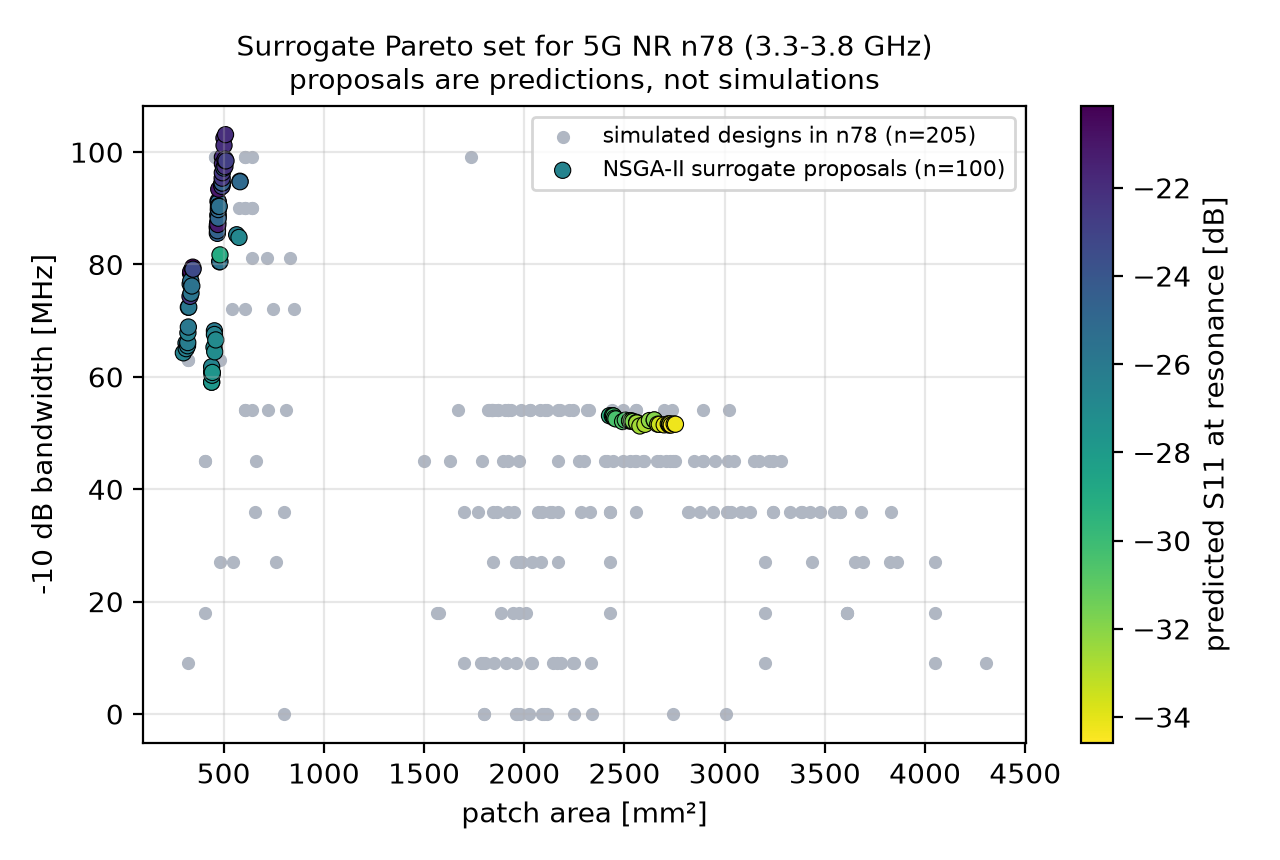
\includegraphics[width=0.76\linewidth]{../results/figures/nsga2_pareto_n78.png}
\caption*{Figure 7. NSGA-II surrogate Pareto set for NR n78 (3.3--3.8 GHz), shown against the simulated designs whose first resonance lies in that band. Proposals are predictions, not simulations.}
\end{figure}
\begin{table}[H]\centering\small
\caption*{Table 8. Three representative Pareto proposals (surrogate predictions, NOT simulated) and their nearest simulated design.}
\begin{tabularx}{\linewidth}{XXXXXXX}
\toprule
\textbf{Proposal} & \textbf{L $\times$ W (mm)} & \textbf{Feed (mm)} & \textbf{Pred. f\_res (GHz)} & \textbf{Pred. S11 (dB)} & \textbf{Pred. BW (MHz)} & \textbf{Nearest simulated (f\_res / S11 / BW)} \\
\midrule
N78-001 (smallest area) & 19.31 $\times$ 15.48 & -2.89 & 3.79 & -26.6 & 64 & P0564: 3.82 / -28.6 / 63 \\
N78-066 (widest BW) & 22.08 $\times$ 23.08 & -4.25 & 3.72 & -22.0 & 103 & P1152: 3.43 / -18.9 / 63 \\
N78-098 (deepest match) & 40.75 $\times$ 67.09 & -1.96 & 3.68 & -34.6 & 51 & P1701: 3.68 / -39.6 / 54 \\
\bottomrule
\end{tabularx}
\end{table}
NSGA-II returned 100 non-dominated proposals (\textbf{E3} -- Met: 100 proposals, median distance to nearest simulated design 0.08 SD (surrogate only, not simulated)). They span 299--2754 mm$^2$, predicted bandwidths of 51--103 MHz and predicted S11 at resonance of -34.6 to -20.1 dB. For comparison, 205 simulated designs resonate in n78; the widest of them has 99 MHz and the smallest covers 320 mm$^2$. The proposals fall into two physically distinct groups: 71 compact patches with L $\approx$ 19--23 mm that use the fundamental mode, and 29 larger patches with L $\approx$ 39--41 mm whose first matched resonance is a higher-order mode, which trade area for a deeper match. The median distance to the nearest simulated design is 0.08 standard deviations, so the proposals are interpolations close to existing data rather than extrapolations. The widest predicted bandwidth (103 MHz) exceeds the best simulated in-band design by less than the surrogate's bandwidth MAE (18 MHz), so no proposal is a demonstrated improvement on the simulated data. That is the expected outcome for a dense sweep of a simple patch; the method becomes valuable when the design space is larger than what was simulated, as with the proposed DGS sweep. No proposal has been simulated, and none should be described as optimal or HFSS-validated. Repeated runs give slightly different Pareto sets because of thread-level non-determinism (docs/REPRODUCIBILITY.md).

\subsection*{9.6 Summary of hypotheses and evaluation criteria}\addcontentsline{toc}{subsection}{9.6 Summary of hypotheses and evaluation criteria}
\begin{table}[H]\centering\small
\caption*{Table 9. Module 2 outcomes.}
\begin{tabularx}{\linewidth}{XXX}
\toprule
\textbf{ID} & \textbf{Statement} & \textbf{Outcome and evidence} \\
\midrule
E1 & Surrogate beats the mean baseline on every patch target (test MAE) & Met: all four targets; weakest s11\_min\_db (4.81 vs 7.36) \\
E2 & Geometry + frequency beats frequency-only (Mendeley, GroupKFold) & Met: S11\_dB 0.533 vs 1.089; Gain 0.513 vs 1.096; Rad\_eff 0.026 vs 0.047 \\
H6 & Fusion (ViT embedding + numeric) > image-only (pre-registered) & Not supported: 0.737 vs 0.775 (numeric-only 0.716) \\
E3 & NSGA-II returns feasible n78 proposals inside the training ranges & Met: 100 proposals, median distance to nearest simulated design 0.08 SD (surrogate only, not simulated) \\
\bottomrule
\end{tabularx}
\end{table}
\section*{10. Ethics, Bias, Privacy, and Reproducibility}\addcontentsline{toc}{section}{10. Ethics, Bias, Privacy, and Reproducibility}
\textbf{Data rights and privacy.} Both datasets are public under licences that permit reuse with attribution (MIT, CC BY 4.0) and contain no personal data. Attribution is given in the LICENSE file, the data card and the references. Raw files are re-downloaded by a script with SHA-256 checks; only derived tables and the Module 1 embeddings are committed.

\textbf{Bias.} (i) Topology and material bias: one coax-fed rectangular patch on one substrate, and one nominal dual-slot design with one-at-a-time variations. (ii) Coverage bias: dense sampling of a small region, so the surrogate is reliable only near simulated designs, as the OOD results show. (iii) Label bias: the -20 dB threshold is an assumption. (iv) Simulation-to-reality gap: no measurements, fabrication tolerances, connector or cable effects. (v) Solver artefacts: implausible Mendeley rows were flagged by a documented rule rather than silently removed.

\textbf{Responsible use.} Surrogate predictions, engineering summaries and Pareto proposals are screening outputs on simulated data. They are labelled as such in every file, and none may be presented as verified antenna performance without full-wave simulation and, for deployment, fabrication and measurement. The text generator is deliberately template-based so that it cannot hallucinate values. The intended scope is civilian communications research.

\textbf{Reproducibility.} One configuration file, fixed seeds, pinned dependencies, dataset revisions and checksums, the locked split manifests shared with Module 1, a provenance file with SHA-256 hashes for the imported embeddings, and scripts for every stage. Ten automated tests cover the S11 target extraction, label thresholds, split integrity against the manifests, the OOD rule, physical ranges, the Mendeley plausibility rule, embedding alignment, the optimisation constraints and the surrogate-versus-baseline check. All ten pass (Appendix D).

\section*{11. Limitations and Future Work}\addcontentsline{toc}{section}{11. Limitations and Future Work}
\begin{itemize}[leftmargin=*,itemsep=1pt]
\item \textbf{Topology mismatch.} The patch data contain no slots or DGS, and the Mendeley data vary one dimension at a time around one design, so the surrogates do not transfer to hybrid-slotted DGS antennas.
\item \textbf{No HFSS.} All targets come from openEMS or the Mendeley authors' solver; HFSS outputs and field quantities were not available.
\item \textbf{Extrapolation.} Tree surrogates fail outside the training ranges (negative OOD R$^2$ for S11 at resonance and bandwidth).
\item \textbf{Matching depth.} S11 depth is predicted only moderately, which limits the reliability of the S11 objective in NSGA-II.
\item \textbf{Fusion.} One embedding run, one seed and no cross-fitting; the result should be confirmed with out-of-fold embeddings.
\item \textbf{Optimisation.} Proposals are unverified, close to existing designs, and the search ignores fabrication constraints and gain.
\end{itemize}
\textbf{Future work.} (1) Generate the HFSS hybrid-slotted DGS sweep described in the reference report with PyAEDT, using a space-filling design of experiments rather than one-at-a-time variation. (2) Retrain the same surrogate pipeline and add uncertainty estimates (quantile forests or Gaussian processes) so that NSGA-II can penalise uncertain regions. (3) Re-simulate the Pareto proposals and add them to the training set in an active-learning loop. (4) Add gain and efficiency objectives once the DGS data provide them for every design. (5) Repeat the fusion experiment with cross-fitted embeddings, several seeds and late-fusion variants. (6) Fabricate and measure a shortlist to quantify the simulation-to-measurement gap.

\section*{12. Conclusion}\addcontentsline{toc}{section}{12. Conclusion}
Module 2 implements and executes a complete, reproducible numerical-text pipeline for the proposed framework. Antenna parameters predict simulated resonance (R$^2$ = 0.89) and bandwidth (R$^2$ = 0.83) well and the depth of the match only moderately (R$^2$ = 0.54) (RQ1); on a slotted patch, the geometry variables roughly halve the error of a frequency-only model for S11, gain and radiation efficiency (RQ2). Fusing numerical features with ViT embeddings did not beat the embeddings alone (0.737 vs 0.775; H6 not supported), but the embeddings themselves reached 0.775, showing that Module 1's representation is stronger than its own classifier head suggests (RQ3). Surrogate-based NSGA-II produced physically interpretable n78 proposals in two mode families, all close to simulated designs and all unverified (RQ4), and the template-based summaries report every prediction next to its simulated reference without inventing values (RQ5). The main lesson for the full HFSS study is that a surrogate is only as good as its coverage: the DGS sweep should be space-filling, the surrogate should report its uncertainty, and every optimised design should be treated as a hypothesis for full-wave verification.

\section*{References}\addcontentsline{toc}{section}{References}
\begin{enumerate}[leftmargin=*,itemsep=1pt]
\item A. Dosovitskiy et al., "An image is worth 16x16 words: Transformers for image recognition at scale," in Proc. ICLR, 2021, arXiv:2010.11929.
\item B. LaBash et al., "Improving generative inverse design of rectangular patch antennas with test time optimization," arXiv:2505.18188, 2025. Dataset: huggingface.co/datasets/becklabash/rectangular-patch-antenna-freq-response (MIT), rev. 4be72a2.
\item M. F. H. Mihad, M. M. Islam and F. H. Sojib, "Antenna Parameters Dataset," Mendeley Data, v2, 2024, doi:10.17632/3gxr2vvd9n.2 (CC BY 4.0).
\item C. A. Balanis, Antenna Theory: Analysis and Design, 4th ed. Hoboken, NJ: Wiley, 2016.
\item 3GPP, "NR; User Equipment (UE) radio transmission and reception; Part 1: Range 1 Standalone," TS 38.101-1.
\item L. Breiman, "Random forests," Machine Learning, vol. 45, no. 1, pp. 5--32, 2001.
\item G. Ke et al., "LightGBM: A highly efficient gradient boosting decision tree," in Proc. NeurIPS, 2017.
\item F. Pedregosa et al., "Scikit-learn: Machine learning in Python," J. Mach. Learn. Res., vol. 12, pp. 2825--2830, 2011.
\item K. Deb, A. Pratap, S. Agarwal and T. Meyarivan, "A fast and elitist multiobjective genetic algorithm: NSGA-II," IEEE Trans. Evol. Comput., vol. 6, no. 2, pp. 182--197, 2002.
\item J. Blank and K. Deb, "pymoo: Multi-objective optimization in Python," IEEE Access, vol. 8, pp. 89497--89509, 2020.
\item T. Liebig et al., openEMS -- a free and open electromagnetic field solver, https://openems.de.
\item A. E. Hoerl and R. W. Kennard, "Ridge regression: Biased estimation for nonorthogonal problems," Technometrics, vol. 12, no. 1, pp. 55--67, 1970.
\item A. Fisher, C. Rudin and F. Dominici, "All models are wrong, but many are useful: Learning a variable's importance by studying an entire class of prediction models simultaneously," J. Mach. Learn. Res., vol. 20, no. 177, pp. 1--81, 2019.
\item D. E. Rumelhart, G. E. Hinton and R. J. Williams, "Learning representations by back-propagating errors," Nature, vol. 323, pp. 533--536, 1986.
\item T. Baltrušaitis, C. Ahuja and L.-P. Morency, "Multimodal machine learning: A survey and taxonomy," IEEE Trans. Pattern Anal. Mach. Intell., vol. 41, no. 2, pp. 423--443, 2019.
\end{enumerate}
\newpage
\section*{Appendix A. Data Dictionary}\addcontentsline{toc}{section}{Appendix A. Data Dictionary}
\begin{table}[H]\centering\small
\caption*{Table 10. Data dictionary (data/data\_dictionary.csv).}
\begin{tabularx}{\linewidth}{XXXXX}
\toprule
\textbf{Dataset} & \textbf{Variable} & \textbf{Type} & \textbf{Unit} & \textbf{Description} \\
\midrule
patch & design\_id & string & - & Unique design key (P + source id) \\
patch & length\_mm & float & mm & Input: patch length L (resonant dimension) \\
patch & width\_mm & float & mm & Input: patch width W \\
patch & feed\_y\_mm & float & mm & Input: coaxial feed offset from patch centre along L (negative toward edge) \\
patch & wl\_ratio & float & - & Input: W/L aspect ratio \\
patch & feed\_ratio & float & - & Input: feed offset normalised by L/2 (0 centre, 1 edge) \\
patch & area\_mm2 & float & mm\textasciicircum{}2 & Patch area W x L (optimisation objective) \\
patch & f\_res\_ghz & float & GHz & Target: first matched resonance, lowest-frequency local S11 minimum below -10 dB (global minimum if never matched) \\
patch & f\_deepest\_ghz & float & GHz & Frequency of the deepest S11 dip in 1-10 GHz (often a higher-order mode) \\
patch & s11\_min\_db & float & dB & Target: global minimum simulated S11 over 1-10 GHz (openEMS FDTD) \\
patch & s11\_at\_res\_db & float & dB & Target: simulated S11 at f\_res \\
patch & bw10\_mhz & float & MHz & Target: contiguous -10 dB bandwidth around f\_res (0 if unmatched) \\
patch & fbw10\_pct & float & \% & Fractional -10 dB bandwidth \\
patch & perf\_class & int & 0/1/2 & Poor (S11min > -10 dB), Acceptable (-20 < S11min <= -10), High (S11min <= -20 dB); fusion target \\
patch & band\_class & int & 0/1/2 & f\_res < 5 GHz | 5-7.125 GHz | >= 7.125 GHz (3GPP FR1 / FR3 boundary) \\
patch & split & category & train/val/test/ood & Locked design-level allocation shared with Module 1 (seed 42) \\
mendeley & design\_id & int & - & Design index (unique combination of the 10 geometry variables) \\
mendeley & Sub\_W, Sub\_L, Sub\_H & float & mm & Input: substrate width, length, height \\
mendeley & Patch\_W, Patch\_L & float & mm & Input: patch width and length \\
mendeley & Feed\_W & float & mm & Input: feed-line width \\
mendeley & Slot1\_W, Slot1\_L, Slot2\_W, Slot2\_L & float & mm & Input: dimensions of the two slots \\
mendeley & Freq\_GHz & float & GHz & Input: frequency at which outputs were extracted (16 values, 1-50 GHz) \\
mendeley & S11\_dB & float & dB & Target: simulated reflection coefficient \\
mendeley & Gain & float & dBi & Target: simulated gain (plausible rows only) \\
mendeley & Rad\_eff & float & ratio & Target: radiation efficiency (plausible rows only) \\
mendeley & Directivity, Total\_eff, VSWR & float & dBi / ratio / - & Other simulated outputs (used for plausibility checks only) \\
mendeley & plausible & bool & - & False if Rad\_eff>1, Total\_eff>1, Directivity>20 dBi or Gain>Directivity \\
\bottomrule
\end{tabularx}
\end{table}
\section*{Appendix B. Configuration}\addcontentsline{toc}{section}{Appendix B. Configuration}
\begin{verbatim}
# Module 2 - Numerical-Text surrogate, multimodal fusion and NSGA-II optimisation.
# Central configuration: every script in src/ reads this file.
seed: 42

paths:
  raw: data/raw
  processed: data/processed
  splits: data/splits
  results: results
  checkpoints: results/checkpoints   # git-ignored (fitted surrogate models)

datasets:
  patch:
    # Hugging Face: becklabash/rectangular-patch-antenna-freq-response (MIT licence)
    repo_id: becklabash/rectangular-patch-antenna-freq-response
    revision: 4be72a22e55fbf46966c59a5d6b3ec95c836379b
    file: data/train-00000-of-00001.parquet
  mendeley:
    # Mendeley Data: Antenna Parameters Dataset, DOI 10.17632/3gxr2vvd9n.2 (CC-BY-4.0)
    dataset_id: 3gxr2vvd9n
    file_url: https://data.mendeley.com/public-files/datasets/3gxr2vvd9n/files/7af017f6-90cd-4da5-a11c-3716378ac3d9/file_downloaded
    sha256: 7c15f2a387d8cc573150f0c361adcaaa74b69d46d30bc63c5a20b23a07dc002a

labels:
  # Matching thresholds. -10 dB (VSWR ~1.92) is the conventional impedance-bandwidth criterion.
  # -20 dB as the "high" boundary is a project ASSUMPTION that requires engineering confirmation.
  s11_matched_db: -10.0
  s11_high_db: -20.0
  # Band edges (GHz) from 3GPP TS 38.101-1 (FR1 upper edge 7.125 GHz; n77 3.3-4.2, n79 4.4-5.0).
  band_edges_ghz: [5.0, 7.125]
  band_names: ["FR1_mid_below5GHz", "FR1_upper_5to7GHz", "FR3_6Gcandidate_above7GHz"]
  perf_names: ["Poor", "Acceptable", "High"]

split:
  # Identical to Module 1: the same locked design-level split (manifests in data/splits).
  train: 0.70
  val: 0.15
  test: 0.15
  ood_wl_ratio_min: 1.95   # widest patches (W/L > 1.95) are an out-of-distribution hold-out

surrogate:
  random_forest_trees: 400
  hist_gbr_iterations: 500
  hist_gbr_learning_rate: 0.05
  ridge_alpha: 1.0
  mendeley_folds: 5          # GroupKFold by design (all 16 frequencies of a design stay together)

fusion:
  # 384-d CLS embeddings exported by Module 1 (pre-registered fine-tuned ViT-S/16, seed 42).
  embedding_run: vit_finetune_patch_perf_class_s42
  embedding_dir: data/external/module1_vit_embeddings
  hidden_grid: [[64], [128, 64]]
  alpha_grid: [1.0e-4, 1.0e-3, 1.0e-2]

nsga2:
  band_ghz: [3.3, 3.8]       # 5G NR n78
  pop_size: 100
  generations: 80

\end{verbatim}
\section*{Appendix C. Experimental Details}\addcontentsline{toc}{section}{Appendix C. Experimental Details}
\begin{table}[H]\centering\small
\caption*{Table 11. Every patch surrogate candidate (validation, test and OOD).}
\begin{tabularx}{\linewidth}{XXXXXXX}
\toprule
\textbf{Target} & \textbf{Model} & \textbf{Val MAE} & \textbf{Test MAE} & \textbf{Test R$^2$} & \textbf{OOD MAE} & \textbf{OOD R$^2$} \\
\midrule
f\_res\_ghz & mean baseline & 1.980 & 1.820 & -0.001 & 2.547 & -0.307 \\
f\_res\_ghz & ridge & 1.150 & 1.117 & 0.602 & 1.562 & 0.436 \\
f\_res\_ghz & random forest & 0.374 & 0.355 & 0.888 & 1.270 & 0.444 \\
f\_res\_ghz & hist gbr & 0.403 & 0.408 & 0.889 & 1.233 & 0.457 \\
s11\_min\_db & mean baseline & 7.345 & 7.363 & -0.000 & 9.474 & -0.393 \\
s11\_min\_db & ridge & 6.389 & 6.403 & 0.253 & 8.265 & 0.017 \\
s11\_min\_db & random forest & 4.712 & 4.815 & 0.538 & 7.305 & 0.132 \\
s11\_min\_db & hist gbr & 5.029 & 5.129 & 0.499 & 5.796 & 0.356 \\
s11\_at\_res\_db & mean baseline & 6.014 & 5.648 & -0.003 & 5.809 & -0.760 \\
s11\_at\_res\_db & ridge & 5.767 & 5.415 & 0.113 & 6.723 & -1.155 \\
s11\_at\_res\_db & random forest & 3.784 & 3.272 & 0.570 & 7.031 & -1.544 \\
s11\_at\_res\_db & hist gbr & 4.002 & 3.513 & 0.497 & 6.045 & -1.056 \\
bw10\_mhz & mean baseline & 59.413 & 55.361 & -0.000 & 47.295 & -1.347 \\
bw10\_mhz & ridge & 47.068 & 47.352 & 0.214 & 57.875 & -4.064 \\
bw10\_mhz & random forest & 17.346 & 18.056 & 0.830 & 38.823 & -3.723 \\
bw10\_mhz & hist gbr & 20.003 & 19.781 & 0.809 & 43.770 & -4.093 \\
\bottomrule
\end{tabularx}
\end{table}
Deviations and abandoned choices: the first definition of resonance (the deepest S11 dip) was replaced before training by the first matched resonance because the deepest dip is often a higher-order mode. Radiation efficiency was added as a Mendeley target when Module 2 was separated from the combined prototype; it uses the same plausibility rule as gain. No test-set result was used for any decision.

\section*{Appendix D. Reproducibility Instructions}\addcontentsline{toc}{section}{Appendix D. Reproducibility Instructions}
\begin{verbatim}
python -m venv .venv && .venv\Scripts\activate
pip install -r requirements.txt
python -m src.download_data          # ~10 MB: patch Parquet + Mendeley XLSX (checksummed)
python -m src.preprocessing          # targets, cleaning, split check against data/splits
python -m src.numerical_model        # surrogates, parity plots, engineering summaries
python -m src.fusion_optimization    # fusion with Module 1 embeddings + NSGA-II
pytest -q
python scripts/make_deliverables.py
\end{verbatim}
Repository: https://github.com/<your-github-username>/module2-numerical-surrogate-antenna-design. The pytest output is stored in results/test\_report.txt; environment and determinism notes are in docs/REPRODUCIBILITY.md.

\end{document}